\subsection{Design method} \label{design_method}
In this research we use the Ampersand method, which is based on relation algebra.
Ampersand makes it possible to make a Conceptual analysis of the source text.
The Conceptual and technical data model created using Ampersand with the descriptions in the Conceptual analysis allows to base the implementation on it.

\subsubsection{Relation Algebra} \label{relation_algebra}
The field of relational algebra focuses on operations on sets, and the signature item of relation algebra is the relationship.
The attributes in the example of \acrshort{big} are the person its surname, first names, gender, date of birth, nationality and address, as well as the number and time of registration~\footnote{\acrlong{big} article 3, paragraph 2 }.
The relation consists of tuples and the relation is between two objects, so one speaks of 2-tuples.
The tuples contain the attributes of the relation.

\begin{samepage}The operations on sets are the following:
\begin{itemize}
    \item Union, $R \cup S$ %vereniging
    \item Intersection, $R \cap S$ %doorsnede
    \item Difference, $R - S$ or $S - R$ %verschil
\end{itemize}
\end{samepage}
A distinction must be made between relation algebra~\citep{maddux_bibliography_2006} and relational algebra~\citep{codd_relational_1970}.
Ampersand uses relation algebra, so it is tuple related.
The relational algebra is the basis of e.g. relational databases which includes projections, selections and joins.
The latter are therefore not part of relation algebra.


\subsubsection{Ampersand} \label{ampersand}
Ampersand is based on relationship algebra and focuses on business rules~\citepNonPub{wedemeijer_l_joosten_smm_michels_garkenbout_jlc_werkboek_ontwerpen_met_bedrijfsregelspdf_nodate} and provides correct information systems.
Our goal is to create a correct and error-free registration system.
Ampersand its other strengths are its support for Conceptual analysis.
It is a platform for reactive programming and generates prototypes.
The Ampersand scripts describe the goals rather than the steps, it is declarative.
We are using Ampersand-v4.6.2 in our research.

Business rules are there to pursue a common goal.
These rules are converted to an information system using the Ampersand method.
The Ampersand method ensures that when a precise set of rules has been established, an information system can be generated.
To learn how Ampersand works in real life, we design a registry in Ampersand that implements the \acrshort{big}~\footnote{\url{https://wetten.overheid.nl/BWBR0006251/2022-04-01/0}}.

\begin{figure}[!h]
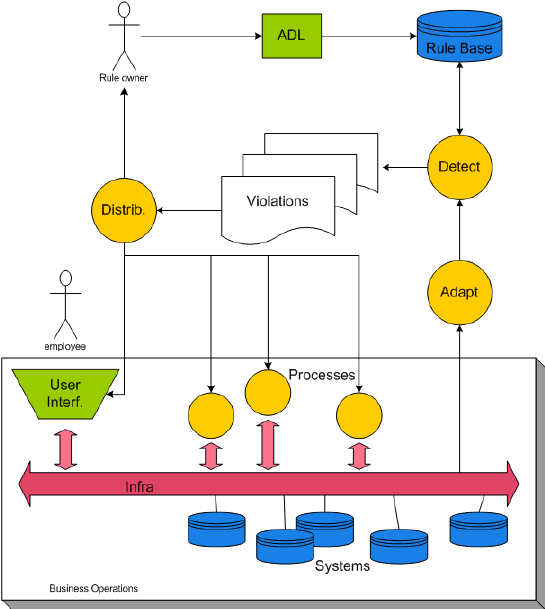
\includegraphics[height=10cm]{Principle-of-rule-based-process-management.png}
\caption{Principle of rule based process-management}
\label{fig:rule-based-proces}
\end{figure}
The principle of rule-based \acrfull{bpm}(see figure~\ref{fig:rule-based-proces}) as mentioned in \citepNonPub{joosten_joosten} is that any violation of a business rule can be used to trigger actions, which is described in the \nameref{reactive_approach} section.

Ampersand describes Concepts that in turn consist of atoms.
An atom is an implementation of the Concept.
Inside the \acrshort{big} is a Concept \textit{Beroep} with associated atoms like \textit{arts}, \textit{tandarts}, etc see listing~\ref{lst:register}, rows 38-48.
We give the Concepts a name so that the Concepts are recognized by the organization.
Recognizability also applies to the definition and purport of the terms.
These attributes are not mandatory, but when one wants to generate a functional design, these descriptions of the attributes are very useful.

Concepts can have relationships with each other.
If the data of the Concepts is true and the rules yield consistent data, then the relationships between real data are facts.
These facts together form one truth.
Not all Concepts are directly related, within the domain of the \acrshort{big} we could distinguish the Concept \textit{Registratie} and the Concept \textit{Beroep}.
These terms come from \url{https://wetten.overheid.nl/BWBR0006251/2022-04-01/0} in article 3 of \acrshort{big}.
\begin{comment}


Even the name of the relationship is mentioned in this article, which the legislator calls a  \textit{beroepsbeoefenaar}. 
The law requires that details of the \textit{registratie} be recorded, stating the corresponding profession.
In Ampersand this is modeled as follows.
On the one hand the \textit{beroep} and also the Concept \textit{registratie}, see listing~\ref{lst:registratie} rows 16-20.

Between the \textit{registratie} and the \textit{persoon} exists the relationship \textit{beroepsbeoefenaar}, see listing~\ref{list:relatie_beroepsbeoefenaar}.
\begin{lstlisting}[language=Octave, caption={Listing RELATION "beroepsbeoefenaar" },captionpos=b, label={list:relatie_beroepsbeoefenaar}] 
RELATION beroepsbeoefenaar [Persoon*Registratie] 
MEANING "geregistreerd persoon"
POPULATION beroepsbeoefenaar CONTAINS 
[
  ("Piet",1);
  ("Susan",2);
  ("Gerard",3);
  ("John",4)
]\end{lstlisting}
By adding the Concepts of \textit{persoon} (see listing~\ref{list:Concept_persoon}) and \textit{handeling} (see listing~\ref{list:Concept_handeling}), people may perform  medical actions, but only when they are qualified.
\begin{lstlisting}[language=Octave, caption={Listing Concept Persoon },captionpos=b, label={list:Concept_persoon}] 
    Concept Persoon "Persoon die werkzaam wilt zijn binnen de zorg"
    PURPOSE Concept Persoon 
    {+Vastleggen van de identiteit van de persoon+}
\end{lstlisting}
\begin{lstlisting}[language=Octave, caption={Listing Concept Handeling },captionpos=b, label={list:Concept_handeling}] 
    Concept Handeling "Acties die uitgevoerd worden" 
    PURPOSE Concept Handeling 
    {+Vastleggen van de mogelijke handelingen die uitgevoerd kunnen worden binnen de zorg+}
\end{lstlisting}
\end{comment}
These Concepts can lead us to the following scheme.
\begin{figure}[H] 
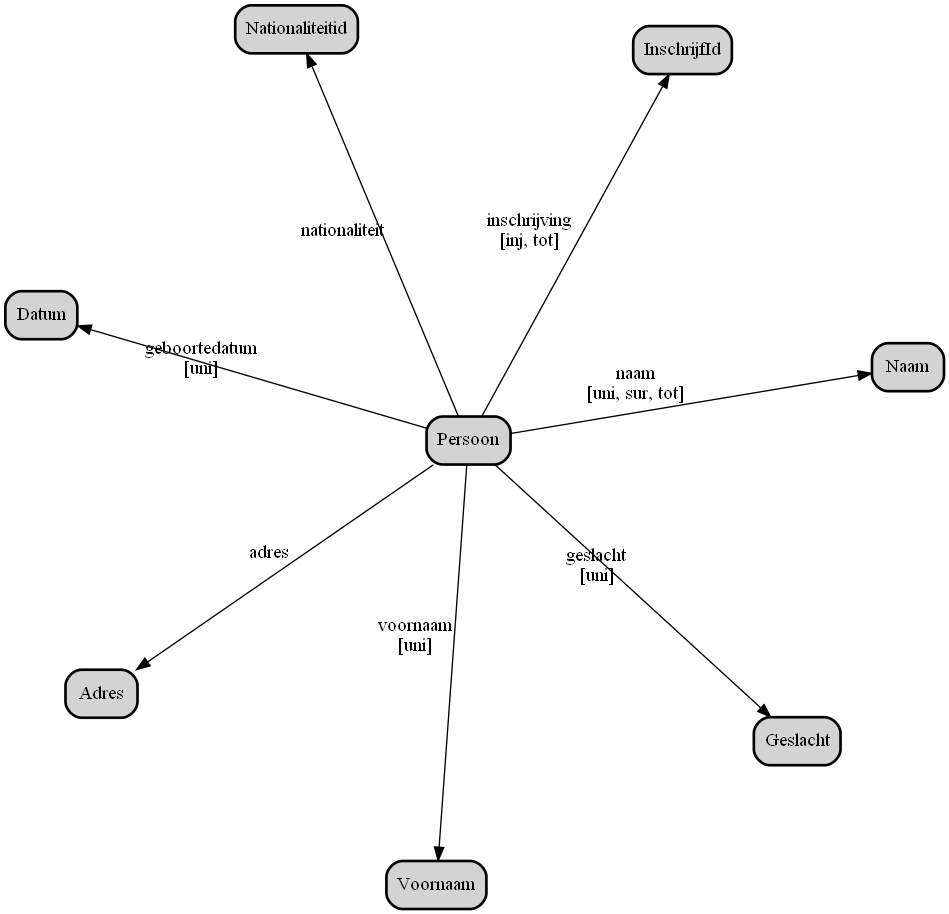
\includegraphics[scale=0.4]{CDConceptPersoon.png}
\centering
\caption{relations of Persoon from \acrshort{ca}}
\label{fig:relations}
\end{figure}


The multiplicity must also be determined for each relation.
For example the relationship between \textit{Persoon} and \textit{Naam}.
\begin{table}[h!]
    \begin{tabular}{||l | l||} 
     \hline
    function & The corresponding control question for the above relation \textit{naam} is\\
    \hline\hline
        Univalent & For each \textit{Persoon} there is at most one \textit{Naam}\\ %elke P max 1 H
        Total & For each \textit{Persoon} there is at least one \textit{Naam} \\ %elke P minimaal 1 H
        Injective & For each \textit{Naam} there is only one \textit{Persoon}, \\&stated that a \textit{Persoon} has a unique \textit{Naam}.\\ %elke H max 1 P 
        Surjection & For each \textit{Handeling} there is at least one \textit{Persoon}. \\&Not possible because of Injective clause.\\ %elke H minimaal 1 P
    \end{tabular}
    \label{tab:multiplicity}
\end{table}

Modeling using the Ampersand method determines which Concepts and Relationships arise within the research case.
Ampersand helps to gain insight into these Relationships.
These Relationships must be recognized by the analyst in the source text and defined in the script.
Ampersand then  generate the \acrshort{ca}  and the prototype.
Using the generated prototype, Ampersand validates the data with constraints on relationships.
This prevents registrations (data) that do not meet the requirements.
These restrictions are defined in rules within Ampersand (see for example listing~\ref{lst:persoon}, rows 39-54).
In figure \ref{fig:relations} the relations are named.
It was previously established that there are 2-tuple relationships.
Here we use the following notation:$\mathit{relation [Concept \times Concept]}$.
\begin{center}
$\mathit{I [Persoon]}$
\newline $\subseteq$
\newline  $\mathit{naam [Persoon \times Naam]}$;
 $\mathit{naam [Persoon \times Naam]~\smallsmile}$
\end{center}
The compared sets are
\newline $\mathit{[Persoon \times Naam]}$
\newline The rule then will determine if the previous equation is true.
\newline If this is the case, then the rule is validated, otherwise the violation message occurs.


\subsection{Reactive approach} \label{reactive_approach}
One of the benefits of Ampersand~\footnote{\url{https://ampersandtarski.gitbook.io/documentation/why-ampersand}} mentioned is the following statement ``Use Ampersand as a platform for reactive programming, to help you of workflows and workflow models.''

This reactive approach by Ampersand starts with the reactive manifest~\citepNonPub{reactive_manifesto}.
The approach in the manifest defines the requirements that a reactive system must meet, such as Responsive, Resilient, Elastic and Message Driven.
These requirements lead to systems that are flexible, loosely coupled, and scalable, making them easier to develop and maintain.
Reactive systems are made highly responsive and provide interactive feedback.
\begin{figure}[H] 
    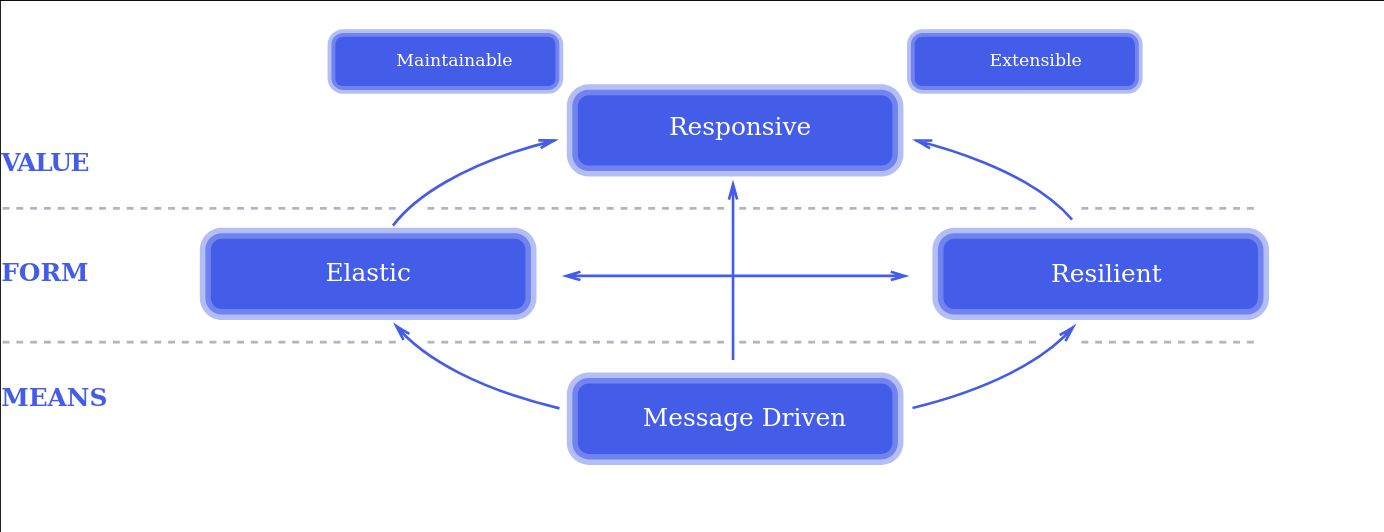
\includegraphics[scale=0.3]{reactive_manifesto.png}
    \centering
    \caption{Reactive Manifesto}
    \label{fig:reactive manifesto}
\end{figure}

Ampersand supports a form of Functional Reactive Programming (FRP)~\citep{elliott_functional_1997}.
The basis of reactive programming is the fact that it involves asynchronous communication.
This means that, as the Reactive Manifesto dictates, it uses message-driven systems, but Ampersand is more than a message-driven system, it is actually an event-driven system.
The glossary of the \citeNonPub{reactive_manifesto} indicates the difference between message-driven systems and event-driven systems.
An event-driven system targets the event bus, while a message-driven system targets recipients~\citep{bainomugisha_survey_2013}.
The essence is that the order of the flow cannot be determined in advance.
The system responds to events caused by constraints and Ampersand determines the dynamic flow~\citep{joosten_relation_2018}.
